\documentclass[cn,11pt,chinese]{elegantbook}

\usepackage{diagbox}
\usepackage{minted}
\usepackage{minted,tabularx,tikz}
\usepackage{graphicx}
\usetikzlibrary{
  shapes,
  shapes.geometric,
  decorations.text,
  shapes.geometric,
  calc,
  decorations.pathreplacing,
  automata,
  positioning,
  arrows
}

\usepackage{tcolorbox}
\tcbuselibrary{skins, breakable, theorems}

\title{尚硅谷Flink教程}
\author{左元}
\date{\today}

\setcounter{tocdepth}{2}

\cover{flink-header-logo.pdf}


% 本文档命令
\usepackage{array}
\newcommand{\ccr}[1]{\makecell{{\color{#1}\rule{1cm}{1cm}}}}

\begin{document}

\maketitle
\frontmatter

\tableofcontents
%\listofchanges

\mainmatter

\chapter{Flink流处理简介}

\begin{introduction}
  \item Flink是什么
  \item 为什么要用Flink
  \item 流处理的发展和演变
  \item Flink的主要特点
  \item Flink vs Spark Streaming
\end{introduction}

\section{Flink是什么}

Apache Flink是一个框架和分布式处理引擎,用于对无界和有界数据流进行状态计算。

有界数据流

Flink会将文件看成一条流,一条一条的处理文件中的数据,例如下面包含两条数据的文本文件,将会一条一条处理,而不会整个文件进行处理。

\begin{lstlisting}[caption={文件流}]
Mary,./home,1970-01-01 00:00:01
Bob,./cart,1970-01-01 00:00:02
\end{lstlisting}

Flink Kafka Consumer,无界数据流,来一条处理一条。

Flink底层引擎对于文件和Kafka消息队列的处理逻辑是一致的。

流批统一,一套业务逻辑代码搞定流和批。

\section{Flink目前在国内企业的应用}

所有大厂都在重度使用Flink。特别是阿里,收购了Flink母公司,并为Flink贡献了海量的代码,双十一大屏的指标全部使用Flink计算。几年前的数据:阿里巴巴每秒钟使用Flink处理4.6PB的数据量。

快手:Flink集群有1500台机器

字节跳动:Apache Storm $\rightarrow$ Apache Flink

Flink对所有的传统的流处理框架是降维打击。

\section{为什么选择Flink}

\begin{itemize}
  \item 流数据更真实地反映了我们的生活方式(点击流)
  \item 传统的数据架构是基于有限数据集的,将数据流人为的变成了离线数据来处理
  \item 我们的目标
    \begin{itemize}
      \item 低延迟(Spark Streaming 的延迟是秒级(需要攒批然后计算),Flink延迟是毫秒级(Spark Streaming的千分之一,Flink是来一条数据就处理一条数据,没有攒批的过程),由于操作系统的时钟的精度是毫秒级,所以可以认为Flink是没有延迟的)
      \item 高吞吐
      \item 结果的准确性和良好的容错性(EXACTLY-ONCE,恰好处理一次,精准一次消费)
    \end{itemize}
\end{itemize}

\begin{tcolorbox}
  Spark Streaming开窗口的大小要求是500毫秒(0.5秒)的整数倍

  延迟的概念:数据到达的时间和得到计算结果的时间的间隔
  
  吞吐的概念:单位时间内能处理的数据量的大小
  
  良好的容错性:程序宕机再重启,计算结果还是正确的。
  
  结果的准确性:某个事件的发生时间是:2020-01-01 00:00:09,
  
  如果我们开一个 10 秒钟的滚动窗口,窗口
  
  窗口一:2020-01-01 00:00:00 $\sim$ 2020-01-01 00:00:10
  
  窗口二:2020-01-01 00:00:10 $\sim$ 2020-01-01 00:00:20
  
  事件由于网络延迟,到达Spark Streaming服务器的时间是:
  
  2020-01-01 00:00:11,被分配到了窗口二中,导致计算结果的不准确。Flink是没有这个问题的。
\end{tcolorbox}

\section{哪些行业需要处理流数据}

\begin{itemize}
  \item 所有行业都需要处理流数据,因为数据本质上是流的形式。
  \item 电商:计算PV(Page View,页面访问次数统计)、UV(Unique Visitor,独立访客统计),以及实时热门商品(每过 5 分钟计算一次过去 1 小时的PV最多的商品)等指标。
  \item 物联网(IoT):温度传感器连续 1 秒钟温度上升的检测。
  \item 风控控制
  \begin{itemize}
    \item 连续三次登录失败的检测(爬虫行为,暴力破解用户名和密码)
    \item 信用卡欺诈检测(连续两笔消费,第一笔消费小于1元,第二笔消费大于500元)
    \item 超时未支付订单的检测(美团下订单,15 分钟未支付,将关闭订单)
    \item 刷单行为(连续三个事件:登录 $\rightarrow$ 下订单 $\rightarrow$ 支付)
  \end{itemize}
\end{itemize}

\section{传统数据处理架构}

\begin{itemize}
  \item OLTP(在线事务处理)
  \item OLAP(在线分析处理)
  \item LAMBDA架构
  \item 有状态的流处理
\end{itemize}

\begin{figure}[htbp]
  \centering
  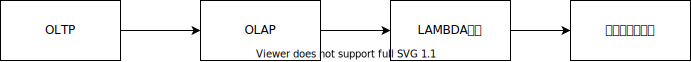
\includegraphics[width=.8\textwidth]{5.pdf}
  \caption{架构演进过程}
\end{figure}

\subsection{OLTP}

用一个关系型数据库完成所有需求。

优点:架构很简单,适合初创公司。

数据库管理员(DBA)负责优化数据库(分库分表,建索引)
\begin{figure}[htbp]
  \centering
  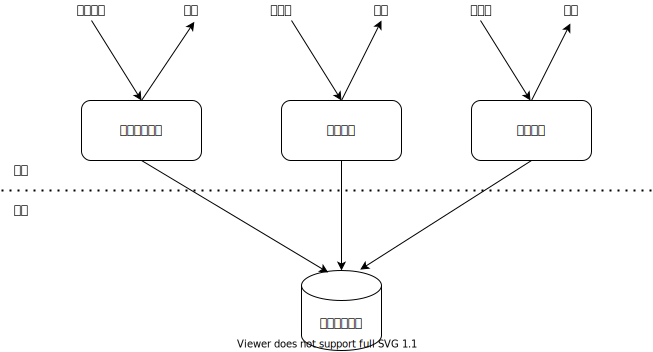
\includegraphics[width=.8\textwidth]{6.pdf}
  \caption{OLTP架构}
\end{figure}

\subsection{OLAP}

优点:解耦合

缺点:得到计算结果的延迟比较大,不够实时

关系型数据库:用户表,用户地址表,订单表

统计指标的计算:Hive

\begin{figure}[htbp]
  \centering
  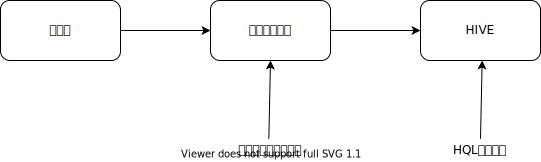
\includegraphics[width=.8\textwidth]{7.pdf}
  \caption{OLAP架构}
\end{figure}

\subsection{LAMBDA架构}

\begin{itemize}
  \item 用两套系统,同时保证低延迟和结果准确性。
  \item 使用批处理框架(hive)保证结果的准确性。但是结果可能会有较大的延迟。
  \item 使用流处理框架(Spark Streaming)保证结果的低延迟。但是结果可能计算的不准确。
\end{itemize}

\begin{figure}[htbp]
  \centering
  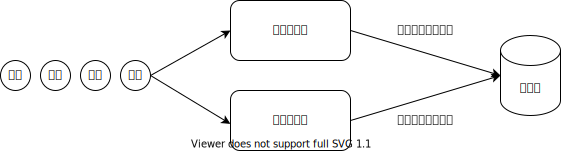
\includegraphics[width=.8\textwidth]{3.pdf}
  \caption{LAMBDA架构}
\end{figure}

例子:

\begin{tcolorbox}
  点击事件:Mary,./Home,1970-01-01 00:00:09

  统计1970-01-01 00:00:00 $\sim$ 1970-01-01 00:00:10窗口的pv指标

  由于存在网络延时,事件在11秒时到达服务器,Spark Streaming可能将数据分到窗口1970-01-01 00:00:10 $\sim$ 1970-01-01 00:00:20

  这样的话,0 $\sim$ 10的统计结果就会少了一条,所以我们可以在晚些时候(例如晚上12点,使用HIVE再来计算一次0 $\sim$ 10窗口的页面访问量,校正一下计算结果,写入数据库)。
  \begin{itemize}
    \item Spark Streaming:保证结果的低延迟,但结果可能不准确
    \item Hive:保证结果的准确性,但结果的延迟比较高
  \end{itemize}

  两套系统计算的指标是同一个指标,所以写的代码也很类似。带来了维护的困难,因为一套代码要写两遍。

  能不能写一份代码就搞定低延迟和结果准确性呢?

  能不能使用一套框架既保证低延迟又保证结果的准确性呢?

  答案就是:Flink。

\end{tcolorbox}

\begin{figure}[htbp]
  \centering
  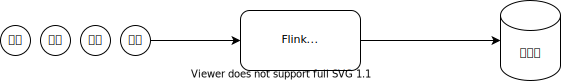
\includegraphics[width=.8\textwidth]{4.pdf}
  \caption{有状态的流处理}
\end{figure}

\section{大数据理论的发展}

\begin{enumerate}
  \item 谷歌三篇论文(2003年):GFS $\rightarrow$ HDFS,MapReduce $\rightarrow$ Hadoop,Big Table $\rightarrow$ HBase
  \item Spark(2008年)、Spark Streaming(将计算场景从磁盘转移到了内存,百倍提升)
  \item 谷歌:Dataflow Model $\rightarrow$ Apache Flink(2015年底)
\end{enumerate}

\section{有状态的流处理}

状态:有些算子可以维护内部状态

流处理:来一条数据处理一条(不攒批)

示意图:来一条数据统计值加一

\begin{enumerate}
  \item 来了一条数据(圆形),触发Flink应用程序的执行
  \item 读取内部状态(统计值)
  \item 统计值加1
  \item 将统计值写回内部状态
  \item 输出统计值(正方形)
\end{enumerate}

从图中可以看出,Flink处理数据是没有落盘操作的。

只在保存检查点(本地状态)的时候落盘。

sum算子中只会维护一个累加器,数据到来更新完累加器之后,数据直接被丢弃掉了。每个key对应的逻辑分区都有一个sum算子。

\begin{figure}[htbp]
  \centering
  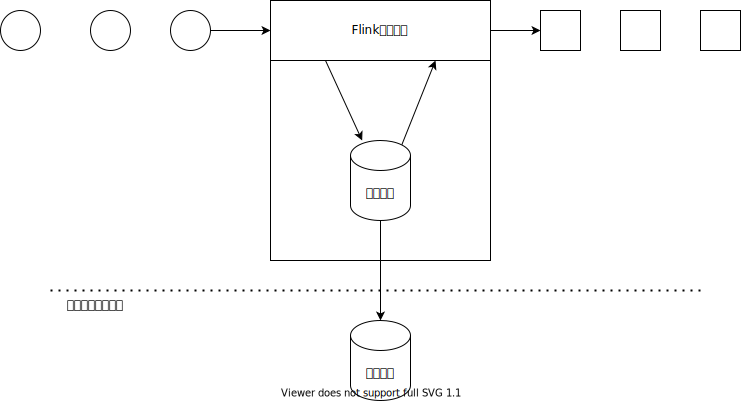
\includegraphics[width=.8\textwidth]{8.pdf}
  \caption{Flink的有状态流处理}
\end{figure}

数据流就像生产流水线

\begin{itemize}
  \item 数据是生产流水线上的产品
  \item 算子是生产流水线上的工人
\end{itemize}

\section{流处理框架的演变}

\begin{itemize}
  \item Apache Storm:低延迟,吞吐量很差,计算结果也不能保证准确性
  \item Apache Spark Streaming:高吞吐,延迟比较高,计算结果也不能保证准确性
  \item Apache Flink
  \begin{itemize}
    \item 低延迟
    \item 高吞吐
    \item 时间正确/语义化窗口
    \item 计算结果的正确性(EXACTLY-ONCE)
  \end{itemize}
\end{itemize}

\section{Flink的主要特点}

\begin{itemize}
  \item 事件驱动
  \item 基于流的世界观
  \item 分层API
  \item 支持事件时间(EventTime)和处理时间(ProcessingTime)语义
    \begin{itemize}
      \item 事件时间(逻辑时钟):事件发生的时间,时间戳包含在事件里
      \item 处理时间(物理时钟):事件到达服务器的机器时间
    \end{itemize}
  \item 精确一次(EXACTLY-ONCE)的状态一致性保证
  \item 低延迟,每秒处理数百万个事件,毫秒级延迟
  \item 与众多常用存储系统的连接(ES,HBase,MySQL,Redis…)
  \item 高可用(Zookeeper),动态扩展,实现7*24小时全天候运行
\end{itemize}

\subsection{事件驱动(Event Driven)}

\begin{itemize}
  \item 来一条数据就处理一次,每来一条数据就会驱动DAG中算子的运行,也可以看作数据在DAG里面流动。
  \begin{figure}[htbp]
    \centering
    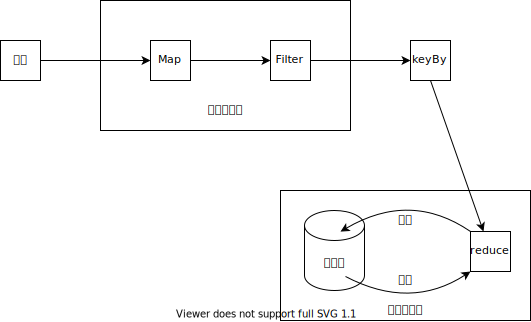
\includegraphics[width=.8\textwidth]{20.pdf}
    \caption{事件驱动示意图}
  \end{figure}
  \item 事件到达之后立即驱动MAP的运行,MAP处理完事件之后,将ETL后的数据发送给FILTER算子,就会立刻驱动FILTER算子的运行,依次类推。
  \item 由于Flink是有状态的流处理,所以可能会有算子会维护和操作内部状态,例如REDUCE算子。而MAP和FILTER是无状态的计算。
  \item 传统批处理示意图如下:
  \begin{figure}[htbp]
    \centering
    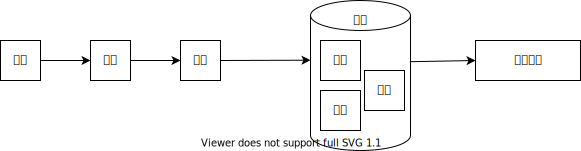
\includegraphics[width=.8\textwidth]{21.pdf}
    \caption{传统批处理示意图}
  \end{figure}
\end{itemize}

\begin{tcolorbox}
\textbf{流处理}

来一条数据处理一条。

flatMap算子什么时候会被触发执行?当flatMap算子的输入到达的时候,触发执行。

sum算子什么时候触发执行呢?当输入数据到达的时候,触发执行。来一条输入数据就要触发一次sum算子的执行。

算子都是被动执行的,数据不来不执行。

这个特性叫做事件驱动,输入事件驱动算子的执行。

生产流水线上的工人,上游的产品到达,触发工人的操作。
\end{tcolorbox}

\subsection{基于流的世界观}

\begin{itemize}
  \item 在Flink的世界观中,一切都是由流组成的,离线数据是有界的流;实时数据是一个没有界限的流:这就是所谓的有界流和无界流。
  \item 在Spark Streaming的世界观中,一切都是由批组成的,离线数据是一批数据;实时数据是无数个微小批次组成的数据。
  \item 流的世界观最重要的一点其实是在静态的离线数据上面加了一个维度:时间
  \item 这个观点来自爱因斯坦的狭义相对论,批处理类似牛顿力学(坐标系:x,y,z),流处理类似狭义相对论力学(坐标系:x,y,z,t)。
\end{itemize}

\subsection{分层API}

\clearpage
\begin{figure}[htbp]
  \centering
  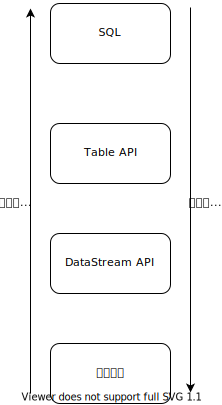
\includegraphics{22.pdf}
  \caption{API层级结构}
\end{figure}

\begin{itemize}
  \item 越抽象,越容易使用,但无法实现复杂的需求。
  \item 越底层,越难掌握,但可以使用很复杂的需求。
  \item 我们的学习重点:DataStream API和底层API。
\end{itemize}

\section{Flink中最重要的两个API}

\textbf{对于单条流的处理}

\begin{tcolorbox}
KeyedProcessFunction
\end{tcolorbox}

\textbf{对于双流JOIN的情况}

\begin{tcolorbox}
CoProcessFunction
\end{tcolorbox}

\section{学习Flink最重要的两个数据结构}

\begin{itemize}
  \item 有向无环图(DAG)
  \item 哈希表(HashMap)
\end{itemize}

\section{Flink中最重要的三个核心概念}

我们在学习Flink时,只需要彻底理解下面三个概念,就能够很好的理解Flink的本质:

\begin{itemize}
  \item 时间语义:事件时间,逻辑时钟(水位线),语义化窗口
  \item 状态:分清有状态的算子和无状态的算子的区别
  \item 事件驱动:来一条数据处理一次,Flink中的算子的计算逻辑都是被动执行的。
\end{itemize}

\section{分布式系统重要概念}

\begin{itemize}
  \item 分区:物理分区和逻辑分区的区别是什么
    \begin{itemize}
      \item hadoop的物理分区:机器节点/容器
      \item hadoop的逻辑分区:每个key对应的分组/分区数据
      \item spark的物理分区:core
      \item spark的逻辑分区:每个key所对应的逻辑分区
      \item flink的物理分区:任务插槽
      \item flink的逻辑分区:每个key所对应的逻辑分区
      \item 同一个逻辑分区的数据,一定在同一个物理分区
      \item 相同key的数据一定在一个节点上
    \end{itemize}
  \item 时钟:物理时钟和逻辑时钟的区别是什么
    \begin{itemize}
      \item flink中的物理时钟:机器时间
      \item flink中的逻辑时钟:水位线
    \end{itemize}
  \item 同步执行和异步执行的区别
    \begin{itemize}
      \item 同步:执行顺序是确定的
      \item 异步:执行顺序是不确定的
        \begin{itemize}
          \item 多进程
          \item 多线程
          \item 单线程异步IO(事件驱动)
        \end{itemize}
    \end{itemize}
\end{itemize}

\section{Flink vs Spark Streaming}

\begin{itemize}
  \item 流 vs 微批
  \item 事件驱动 vs 非事件驱动
  \item 数据模型
    \begin{itemize}
      \item Spark:RDD,Spark Streaming 的 DStream 实际上也就是一组组小批数据 RDD 的集合。
      \item Flink 基本数据模型是数据流,以及事件(Event)序列(Integer、String、Long、POJO Class、Tuple)
    \end{itemize}
  \item 运行时架构
    \begin{itemize}
      \item Spark是批计算,将DAG划分为不同的Stage,一个Stage完成后才可以计算下一个Stage。
      \item Flink是标准的流执行模式,一个事件在一个节点处理完后可以直接发往下一个节点进行处理。
    \end{itemize}
  \item Spark Streaming的延迟是Flink的1000倍。
  \item Flink支持事件时间和处理时间,Spark Streaming只支持处理时间
  \item Flink支持会话窗口
\end{itemize}

\section{Flink程序的典型结构}

\begin{enumerate}
  \item 获取流执行环境
  \item 设置并行任务的数量
  \item 读取数据源
  \item 进行计算
  \item 输出
  \item 执行程序
\end{enumerate}

\chapter{Flink运行时架构}

\section{Flink主从架构}

\begin{itemize}
  \item Flink 运行时由两种类型的进程组成:一个JobManager(作业管理器,Master进程)和一个或者多个TaskManager(任务管理器,Slave进程)。
  \item 典型的Master-Slave(主从)架构。
\end{itemize}

\begin{figure}[htbp]
  \centering
  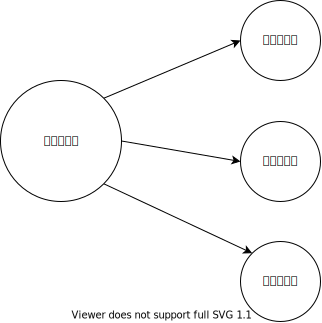
\includegraphics{23.pdf}
  \caption{Flink的主从架构}
\end{figure}

\section{作业管理器}

作业管理器是一个 JVM 进程。进程中包含三类线程:

\begin{itemize}
  \item Flink的资源管理器(ResourceManager):资源是任务插槽(Task Slot)
  \item 分发器(WebUI):提交任务和监控集群和任务
  \item JobMaster(每个作业对应一个):调度任务,将DAG部署到任务管理器
\end{itemize}

\clearpage
\begin{figure}[htbp]
  \centering
  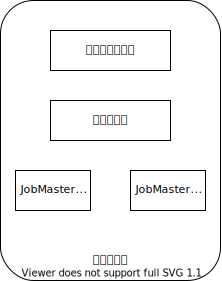
\includegraphics{24.pdf}
  \caption{作业管理器的三种线程}
\end{figure}

JobMaster由于是每个作业对应一个,所以可能有多个JobMaster线程。

\section{任务管理器}

\begin{itemize}
  \item 任务管理器也是一个JVM进程。包含至少一个任务插槽。
  \item 任务插槽是Flink的最小计算单元。
  \item 任务插槽(Task Slot):是一个物理分区。
  \item 每个任务插槽是一个内存分片,每个任务插槽占用一段内存。
  \item 一个任务插槽中至少运行一个线程。
  \item 任务插槽内存大小 = 堆内存 / 任务插槽数量
\end{itemize}

\section{任务插槽}

\begin{itemize}
  \item 不同算子的并行子任务可以共享同一个任务插槽。
  \item 相同算子的不同并行子任务不能共享同一个任务插槽。
  \item 算子的并行度是N,那么算子就有N个并行子任务,并且必须占用N个任务插槽。
\end{itemize}

\begin{figure}[htbp]
	\centering
	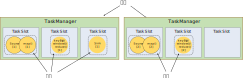
\includegraphics[width=.8\textwidth]{tasks_slots.pdf}
  \caption{每个slot一个线程的情况}
\end{figure}

\begin{figure}[htbp]
	\centering
	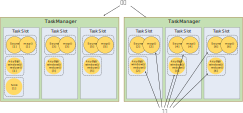
\includegraphics[width=.8\textwidth]{slot_sharing.pdf}
  \caption{每个slot多个线程的情况}
\end{figure}

\begin{figure}[htbp]
  \centering
  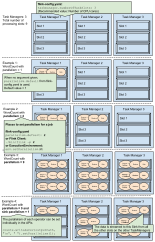
\includegraphics[height=.8\textheight]{slots_parallelism.pdf}
  \caption{任务槽数量和并行度数量的关系}
\end{figure}

\section{并行度的设置}

并行度指的是算子的并行度。

算子并行度的大小不能超过集群可用任务插槽的数量。

从上到下,优先级升高。

\begin{enumerate}
  \item 任务管理器的配置文件里面:flink-conf.yaml中的配置项parallelism.default: 1
  \item 在命令行提交任务时指定并行度:./bin/flink run jar包 -p 16
  \item 全局并行度:env.setParallelism(1)
  \item 针对算子设置并行度:.print().setParallelism(1)
\end{enumerate}

\section{并行度设置的最佳实践}

\begin{enumerate}
  \item 不要设置全局并行度,因为没办法在命令行做动态扩容。
  \item 针对某些算子设置并行度,例如数据源,为了不改变数据的顺序,设置数据源的并行度为1。
  \item 在命令行设置,可以动态扩容
\end{enumerate}

\section{任务提交流程}

\begin{figure}[htbp]
  \centering
  \input{figure/13.pdf_tex}
  \caption{Flink任务提交流程}
\end{figure}

\begin{enumerate}
  \item 在集群启动时,任务管理器会向资源管理器注册自己的任务插槽
  \item 任务管理器之间存在数据的交换
\end{enumerate}

\section{Flink中的DAG数据结构}

\begin{figure}[htbp]
  \centering
  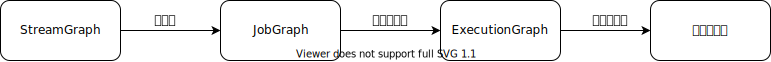
\includegraphics[width=.2\textwidth]{9.pdf}
  \caption{Flink中DAG数据结构的转换}
\end{figure}

\begin{itemize}
  \item StreamGraph:是根据用户通过Stream API编写的代码生成的最初的有向无环图。用来表示程序的拓扑结构。
  \item JobGraph:StreamGraph在编译的阶段经过优化后生成了JobGraph,提交给 JobManager的数据结构。主要的优化为,将多个符合条件(没有shuffle,并行度相同)的算子串在一起作为一个任务链节点。保证同一个任务链节点里面的所有算子都在同一个任务插槽的同一个线程中执行。这样算子之间的数据就是本地转发(无需序列化反序列化和网络IO)两个条件:
    \begin{itemize}
      \item 两个算子之间没有shuffle存在
      \item 两个算子的并行度必须相同
    \end{itemize}
  \item ExecutionGraph:JobManager根据JobGraph生成ExecutionGraph。ExecutionGraph是JobGraph的并行化版本,是调度层最核心的数据结构。
  \item 物理执行图:JobManager根据ExecutionGraph对Job进行调度后,在各个 TaskManager上部署Task后形成的“图”,并不是一个具体的数据结构。
\end{itemize}

我们看一下如下伪代码的DAG是如何进行转换的。

\begin{lstlisting}
source.setParallelism(1)
      .flatMap().setParallelism(2)
      .keyBy()
      .reduce().setParallelism(2)
      .sink().setParallelism(2)  
\end{lstlisting}

首先生成的是StreamGraph。

\begin{figure}[htbp]
  \centering
  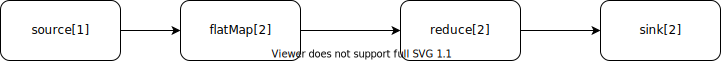
\includegraphics[width=.8\textwidth]{10.pdf}
  \caption{StreamGraph}
\end{figure}

StreamGraph在客户端编译时生成了JobGraph。

\begin{itemize}
  \item source和flatMap由于并行度不同,所以无法合并成一个任务链。
  \item flatMap和reduce虽然并行度相同,但由于算子之间存在shuffle,所以也无法合并成一个任务链。
  \item reduce和sink并行度相同,且不存在shuffle,所以可以合成一个任务链。
\end{itemize}

\begin{figure}[htbp]
  \centering
  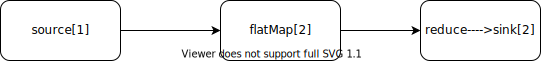
\includegraphics[width=.8\textwidth]{11.pdf}
  \caption{JobGraph}
\end{figure}

将JobGraph提交到作业管理器,会生成ExecutionGraph,也就是将算子按照并行度拆分成多个并行子任务。

\begin{figure}[htbp]
  \centering
  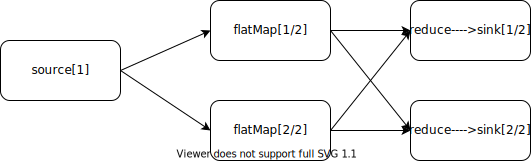
\includegraphics[width=.8\textwidth]{12.pdf}
  \caption{ExecutionGraph}
\end{figure}

JobMaster将ExecutionGraph部署到TaskManager执行。

\chapter{DataStream API}

\section{自定义数据源}

\subsection{POJO CLASS}

\begin{enumerate}
  \item 必须是公有类
  \item 所有字段必须是公有字段
  \item 必须有空构造器
\end{enumerate}

\subsection{SourceFunction}

SourceFunction<T>的泛型是数据源中的数据的类型。

\begin{itemize}
  \item run方法用来发送数据
  \item cancel方法在取消任务时执行
\end{itemize}

\begin{note}
  编写Flink程序时,要注意泛型和方法的参数类型!
\end{note}

其他自定义数据源API

\begin{itemize}
  \item ParallelSourceFunction<T>:并行数据源
  \item RichSourceFunction<T>:富函数版本
  \item RichParallelSourceFunction<T>:并行数据源的富函数版本
\end{itemize}

\section{基本转换算子}

基本转换算子都是\textbf{无状态算子}。

用在keyBy之前。

举个无状态函数的例子

\begin{lstlisting}
      int add(int n) {
        return n + 1;
      }
\end{lstlisting}

在输入相同的情况下,输出一定相同。

\begin{itemize}
  \item MapFunction<IN, OUT>的语义:针对流或者列表中的每一个元素,输出一个元素
  \item FlatMapFunction<IN, OUT>的语义:针对流或者列表中的每个元素,输出0个、1个或者多个元素
  \item FilterFunction<IN>的语义:针对流或者列表中的每个元素,输出0个或者1个元素
\end{itemize}

flatMap是map和filter的泛化,也就是说可以使用flatMap来实现map和filter的功能。

\section{逻辑分区算子}

\begin{itemize}
  \item keyBy做的两件事情:
  \begin{itemize}
    \item 指定数据的key。
    \item 根据key计算出数据要去的任务插槽。
  \end{itemize}
  \item 相同key的数据一定在同一个任务插槽(物理分区)中
  \item 不同key的数据也可能在同一个任务插槽(物理分区)中
  \item 同一个逻辑分区的数据一定在同一个物理分区中。
\end{itemize}

\begin{note}
  keyBy不是一个算子,因为不具备计算功能。keyBy的作用只是为数据指定key,并将数据路由到对应的逻辑分区。
\end{note}

reduce是有状态算子。举个有状态函数的例子。

\begin{lstlisting}
      int count = 0;
      int add(int n) {
        count += n;
        return count;
      }
\end{lstlisting}

输入相同的情况下,输出不一定相同。

\begin{itemize}
  \item ReduceFunction<T>的语义:reduce会初始化一个空累加器(类型和流中的元素类型相同),第一条元素到来,直接作为累加器保存,并将累加器输出。第二条以及之后的元素到来,和累加器进行累加操作并更新累加器,然后将累加器输出。reduce函数定义的是输入元素和累加器的累加规则。
  \item 每个key都会维护自己的累加器,输入数据更新完累加器之后,直接被丢弃
  \item reduce只能在keyBy之后使用。
\end{itemize}

\subsection{reduce算子如何维护逻辑分区}

\begin{figure}[htbp]
  \centering
  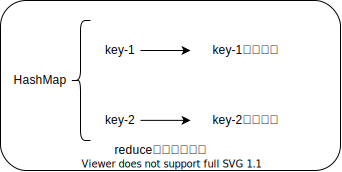
\includegraphics[width=.8\textwidth]{15.pdf}
  \caption{reduce算子的并行子任务如何维护逻辑分区}
\end{figure}

假设我们有如下Flink代码:

\begin{lstlisting}
  env
    // fromElements继承全局并行度为1
    .fromElements(1,2,3,4,5,6,7,8)
    .keyBy(r -> r % 3)
    .sum(0).setParallelism(4)
    .print().setParallelism(4);
\end{lstlisting}

那么keyBy对数据的路由方式可能是:

\begin{figure}[htbp]
  \centering
  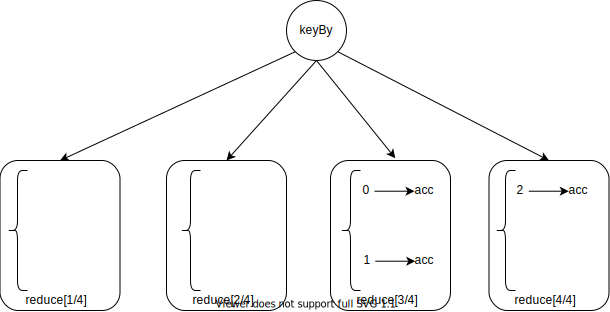
\includegraphics[width=.8\textwidth]{14.pdf}
  \caption{keyBy可能的一种路由方式}
\end{figure}

\section{物理分区算子}

将数据分发到不同的任务插槽(物理分区)

\begin{itemize}
  \item shuffle():随机向下游的并行子任务发送数据。
  \item rebalance()
  \item rescale()
  \item broadcast()
  \item global()
  \item custom()
\end{itemize}

\section{富函数}

生命周期(对象的生命周期,html页面的生命周期,锁的生命周期,数据库连接的生命周期,...)

算子的每一个并行子任务(任务槽)都有自己的生命周期。

\begin{itemize}
  \item open方法:在算子的计算逻辑执行前执行一次,适合做一些初始化的工作(打开一个文件,打开一个网络连接,打开一个数据库的连接)
  \item close方法:在算子的计算逻辑执行完毕之后执行一次,适合做一些清理工作。(关闭一个文件,关闭网络连接,关闭数据库连接)
  \item getRuntimeContext()方法:用来获取算子运行时的一些上下文信息。比如当前算子所处的并行子任务的索引等等。
\end{itemize}

举一些例子

\begin{itemize}
\item MapFunction $\rightarrow$ RichMapFunction
\item FilterFunction $\rightarrow$ RichFilterFunction
\item FlatMapFunction $\rightarrow$ RichFlatMapFunction
\item SourceFunction $\rightarrow$ RichSourceFunction
\item SinkFunction $\rightarrow$ RichSinkFunction
\end{itemize}

\section{自定义输出}

SinkFunction<T>:泛型是要输出的数据的泛型

\chapter{底层API}

底层API(处理函数)都是富函数。

\section{ProcessFunction}

针对没有keyBy的数据流,可以使用ProcessFunction接口,针对流中的每个元素输出0个、1个或者多个元素。(非常类似RichFlatMapFunction)

\begin{itemize}
  \item ProcessFunction<IN, OUT>:IN是输入的泛型,OUT是输出的泛型
  \item processElement:每来一条数据,调用一次
  \item 使用.process(new ProcessFunction<I, O>)来调用。
\end{itemize}

\section{KeyedProcessFunction}

针对keyBy之后的键控流(KeyedStream),可以使用KeyedProcessFunction

\begin{itemize}
  \item KeyedProcessFunction<KEY, IN, OUT>:KEY是key的泛型,IN是输入的泛型,OUT是输出的泛型。
  \item processElement:来一条数据,触发调用一次。
  \item onTimer:定时器。时间到达某一个时间戳触发调用。
  \begin{figure}[htbp]
    \centering
    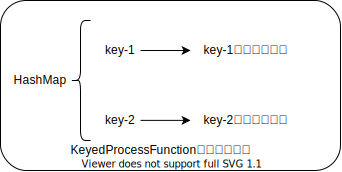
\includegraphics[width=.8\textwidth]{16.pdf}
    \caption{KeyedProcessFunction的并行子任务如何维护定时器}
  \end{figure}
  \item 每个key都会维护自己的定时器,每个key都只能访问自己的定时器。就好像每个key都只能访问自己的累加器一样。
  \item 针对每个key,在某个时间戳只能注册一个定时器,定时器不能重复注册,如果某个时间戳已经注册了定时器,那么再对这个时间戳注册定时器就不起作用了。
  \item .registerProcessingTimeTimer(ts):在机器时间戳ts注册了一个定时器(onTimer)。
  \item 维护的内部状态
    \begin{itemize}
      \item 状态变量
      \item 定时器
    \end{itemize}
  \item processElement方法和onTimer方法:这两个方法是原子性的,无法并发执行。某个时刻只能执行一个方法。因为这两个方法都有可能操作相同的状态变量。例如:到达了一个事件,此时onTimer正在执行,则必须等待onTimer执行完以后,再调用processElement。再比如:到达了一个水位线,想触发onTimer,但此时processElement正在执行,那么必须等待processElement执行完以后再执行onTimer。
  \item 当水位线到达KeyedProcessFunction,如果这条水位线触发了onTimer的执行,则必须等待onTimer执行完以后,水位线才能向下游发送。
  \item 当水位线到达ProcessWindowFunction,如果这条水位线触发了process方法的执行,则必须等待process方法执行完以后,水位线才能向下游发送。
\end{itemize}

\begin{note}
  在KeyedProcessFunction中,可以认为维护了多张HashMap,每个状态变量的定义都会初始化一张HashMap,同时还有一张维护每个key的定时器队列的HashMap。
\end{note}

\section{逻辑分区维护的状态-键控状态变量}

每个key都会维护自己的状态变量

\begin{itemize}
  \item ValueState:类似Java的普通变量一样使用。
  \item ListState:类似Java的ArrayList一样使用。
  \item MapState:类似Java的HashMap一样使用。
\end{itemize}

\subsection{ValueState-值状态变量}

\begin{enumerate}
  \item 每个key都只能访问自己的状态变量,状态变量是每个key独有的。
  \item 状态变量是单例,只能被初始化一次。
  \item 状态变量会每隔一段时间作为检查点保存到状态后端(例如HDFS)。
  \item 当Flink程序启动时,会先去状态后端(例如HDFS)寻找状态变量,如果找不到,则初始化。如果找到了,则直接读取。所以说是单例。为什么Flink程序启动的时候,先去状态后端寻找状态变量呢?因为Flink不知道程序是第一次启动,还是故障恢复启动。如果是故障恢复,则要去保存的检查点里寻找状态变量,恢复到最近一次检查点的状态。
  \item .getState方法通过状态描述符去状态后端寻找状态变量
  \item 读取值状态变量中的值:.value()方法
  \item 将值写入状态变量:.update()方法
  \item 如何清空状态变量:.clear()方法
\end{enumerate}

\clearpage
\begin{figure}[htbp]
  \centering
  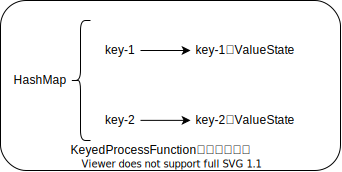
\includegraphics[width=.8\textwidth]{17.pdf}
  \caption{KeyedProcessFunction的并行子任务如何维护ValueState}
\end{figure}

\subsection{ListState-列表状态变量}

\begin{itemize}
  \item .get()方法:返回包含列表状态变量中所有元素的迭代器
  \item .clear()方法:清空状态变量
  \item .add()方法:添加元素
\end{itemize}

\begin{figure}[htbp]
  \centering
  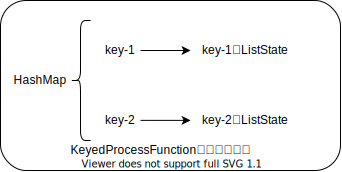
\includegraphics[width=.8\textwidth]{19.pdf}
  \caption{KeyedProcessFunction的并行子任务如何维护ListState}
\end{figure}

\subsection{MapState-字典状态变量}

\begin{itemize}
  \item .put(KEY, VALUE)方法:添加KEY $\rightarrow$ VALUE键值对
  \item .get(KEY)方法:获取KEY的VALUE
  \item .contains(KEY)方法:检测KEY是否存在
  \item .keys():返回所有KEY组成的集合
\end{itemize}

\clearpage
\begin{figure}[htbp]
  \centering
  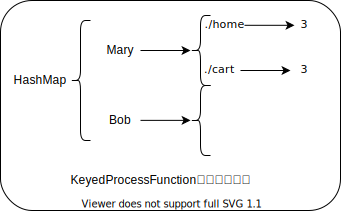
\includegraphics[width=.8\textwidth]{18.pdf}
  \caption{KeyedProcessFunction的并行子任务如何维护MapState}
\end{figure}

\section{窗口API}

\subsection{ProcessWindowFunction}

使用在stream.keyBy().window()之后的流

\begin{itemize}
  \item ProcessWindowFunction<IN, OUT, KEY, WINDOW>
  \item process方法:窗口闭合的时候触发调用
  \item Flink中的窗口是左闭右开:[0,10),当时间到达9999ms的时候,触发process函数的调用。
  \item 窗口从1970-01-01 00:00:00开始对齐
  \item 滚动窗口的计算公式,开了一个10秒钟的滚动窗口,7秒钟到达的事件属于哪个窗口?
  \item 窗口开始时间 = 时间戳 - 时间戳 \;\% 窗口大小
  \item 属于某个窗口的第一条数据到达以后才会开窗口
  \item 窗口内部状态:
    \begin{itemize}
      \item 属于窗口的所有事件
      \item 定时器:时间戳=窗口结束时间 - 1毫秒(因为是左闭右开区间),方法是process函数
    \end{itemize}
\end{itemize}

\begin{tcolorbox}
  在只使用ProcessWindowFunction的情况下,process方法的迭代器参数包含了属于窗口的所有数据,会对内存造成压力,那么应该怎么去优化呢?使用累加器的思想。
\end{tcolorbox}

\subsection{AggregateFunction}

增量聚合函数,关键思想是在每个窗口中维护一个累加器。

\begin{itemize}
  \item AggregateFunction<IN, ACC, OUT>
  \item createAccumulator:创建空累加器,返回值的泛型是累加器的泛型
  \item add:定义输入数据和累加器的聚合规则,返回值是聚合后的累加器
  \item getResult:窗口闭合时发出聚合结果,返回值是将要发送的聚合结果
\end{itemize}

\subsection{将AggregateFunction和ProcessWindowFunction结合使用}

当窗口闭合时:AggregateFunction将getResult()方法的返回值,发送给了ProcessWindowFunction。

\begin{figure}[htbp]
  \centering
  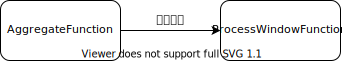
\includegraphics[width=.8\textwidth]{25.pdf}
  \caption{AggregateFunction将getResult的结果发送给ProcessWindowFunction}
\end{figure}

ProcessWindowFunction的process方法的迭代器参数中只有一个元素。

\subsection{窗口的底层实现}

\textbf{AggregateFunction和ProcessWindowFunction结合使用的底层实现}

\begin{figure}[htbp]
  \centering
  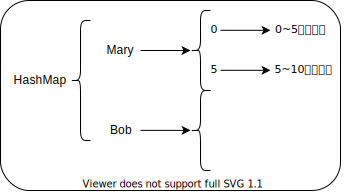
\includegraphics[width=.8\textwidth]{26.pdf}
  \caption{AggregateFunction和ProcessWindowFunction结合使用}
\end{figure}

\textbf{只使用ProcessWindowFunction的底层实现}

\clearpage
\begin{figure}[htbp]
  \centering
  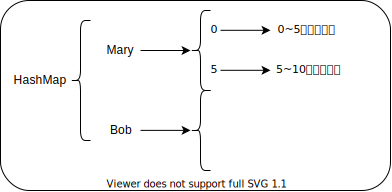
\includegraphics[width=.8\textwidth]{27.pdf}
  \caption{只使用ProcessWindowFunction}
\end{figure}

窗口中的所有元素都保存在List中。

\subsection{ProcessAllWindowFunction}

\begin{lstlisting}
stream
  .windowAll()
  .process(new ProcessAllWindowFunction())
\end{lstlisting}

直接对流进行开窗口,等价于将所有数据keyBy到同一条流,然后进行开窗口

\begin{lstlisting}
stream
  .keyBy(r -> 1)
  .window()
  .process(new ProcessWindowFunction())
\end{lstlisting}

\subsection{触发器}

\begin{lstlisting}
stream
  .keyBy()
  .window()
  .trigger()
  .process()/aggregate()
\end{lstlisting}

触发器触发的是trigger后面的process/aggregate方法。

Trigger<T, W>:T是窗口中的元素类型,W是窗口类型。

TriggerResult

\begin{itemize}
  \item CONTINUE
  \item FIRE
  \item PURGE
  \item FIRE\_AND\_PURGE
\end{itemize}

Trigger中的核心方法

\begin{itemize}
  \item onElement:每来一条数据调用一次
  \item onProcessingTime:处理时间定时器
  \item onEventTime:事件时间定时器
  \item clear:窗口闭合时触发调用
\end{itemize}

\chapter{窗口}

\section{窗口概念}

\begin{itemize}
  \item 一般真实的流都是无界的,怎样处理无界的数据?
  \item 可以把无限的数据流进行切分,得到有限的数据集进行处理—也就是得到有界流
  \item 窗口(Window)就是将无限流切割为有限流的一种方式,它会将流数据分发到有限大小的桶(bucket)中进行分析
\end{itemize}

\section{窗口的本质}

我们一般在.keyBy之后使用.window方法来进行开窗,实际上是在keyBy之后的逻辑分区中,再按照窗口进行一次逻辑分区。先分流再开窗。

\begin{lstlisting}
SELECT * FROM table GROUP BY key, window;
\end{lstlisting}

Flink窗口是左闭右开的区间,例如[0, 5)的窗口最后一个时间戳是4999毫秒。

\section{窗口类型}

\begin{itemize}
  \item 时间窗口(Time Window)
    \begin{itemize}
      \item 滚动时间窗口
      \item 滑动时间窗口
      \item 会话窗口
    \end{itemize}
  \item 计数窗口(Count Window)
    \begin{itemize}
      \item 滚动计数窗口
      \item 滑动计数窗口
    \end{itemize}
\end{itemize}

\section{滚动窗口}

\begin{itemize}
  \item 将数据依据固定的窗口长度对数据进行切分
  \item 时间对齐,窗口长度固定,没有重叠
\end{itemize}

\clearpage
\begin{figure}[htbp]
  \centering
  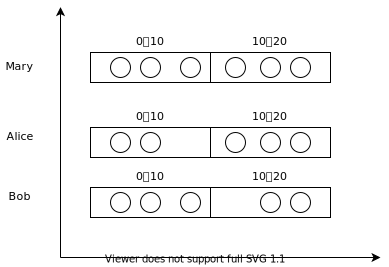
\includegraphics[width=.8\textwidth]{28.pdf}
  \caption{滚动窗口}
\end{figure}

\section{滑动窗口}

\begin{figure}[htbp]
  \centering
  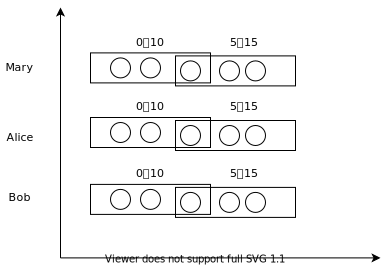
\includegraphics[width=.8\textwidth]{29.pdf}
  \caption{滑动窗口}
\end{figure}

\begin{itemize}
  \item 滑动窗口是固定窗口的更广义的一种形式,滑动窗口由固定的窗口长度和滑动间隔组成
  \item 窗口长度固定,可以有重叠
  \item 如果一个元素同时属于两个窗口,那么会将元素复制两份,每个窗口分配一个元素。这样就可以保证所有的窗口从逻辑上分开处理。
\end{itemize}

\section{会话窗口}

\begin{itemize}
  \item 会话窗口的长度是不固定的。
  \item 使用超时时间来定义会话窗口。
\end{itemize}

\begin{figure}[htbp]
	\centering
	
\includegraphics[width=.8\textwidth]{30.pdf}
  \caption{会话窗口}
\end{figure}

\chapter{逻辑时钟-水位线}

两种时间语义

\begin{figure}[htbp]
  \centering
  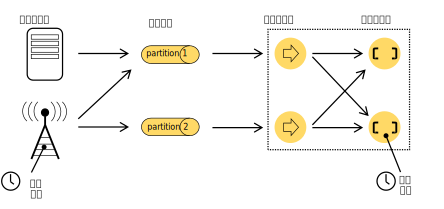
\includegraphics[width=.8\textwidth]{figure/event_processing_time.pdf}
  \caption{两种时间语义}
\end{figure}

\begin{itemize}
  \item 处理时间:事件进入process算子的时间。
  \item 事件时间:事件中包含的时间戳,事件真实发生的时间。
\end{itemize}

举两个例子:

\begin{figure}[htbp]
  \centering
  
\includegraphics[width=.8\textwidth]{31.pdf}
  \caption{星球大战}
\end{figure}

\clearpage
\begin{figure}[htbp]
  \centering
  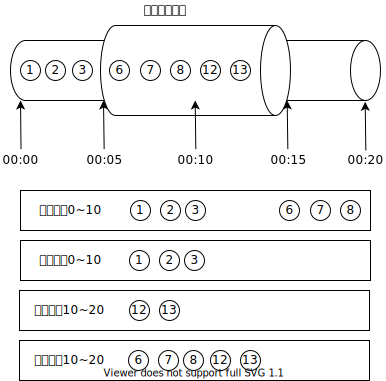
\includegraphics[width=.8\textwidth]{34.pdf}
  \caption{打游戏}
\end{figure}

由于事件时间的世界里面没有时钟,所以我们需要为这个世界提供时钟,叫做水位线(逻辑时钟)。

时钟的定义:单调递增的序列。

如果单调递增的序列是CPU产生的,那么就是物理时钟。如果是编程产生的,那么就是逻辑时钟。

水位线流动到哪一个算子,哪一个算子就会更新自己的时钟(产线工人的手表)。水位线不会弯道超车,也就是说,水位线不会绕过水位线前面的数据传播下去。如果某个算子的计算过程很耗时,那么会阻塞水位线的向下传播。如果上游的算子阻塞了水位线的传播,那么上游算子和下游算子的水位线(时钟)可能是不一样的。

在使用处理时间(ProcessingTime)的情况下,不存在乱序数据的情况。

乱序数据只存在于使用事件时间的情况下。

时钟:

\begin{itemize}
  \item 物理时钟:机器时间,墙上时钟
  \item 逻辑时钟:水位线
\end{itemize}

在Flink里面,时钟的作用是什么?

\begin{itemize}
  \item 触发定时器
  \item 关闭窗口
\end{itemize}

\section{有关水位线的一些约定}

\begin{theorem}{}{}
  水位线是事件时间的世界中的逻辑时钟。
\end{theorem}

\begin{theorem}{}{}
  Flink认为携带时间戳 $\le$ 水位线的事件都已经到达。
\end{theorem}

\begin{theorem}{}{}
  水位线是一种特殊的事件。由程序员编程插入到数据流中。随数据流流动。
\end{theorem}

\begin{theorem}{}{}
  算子的每个并行子任务会维护自己的逻辑时钟,当接收到上游发送过来的水位线时,更新自己的逻辑时钟。
\end{theorem}

\begin{theorem}{}{}
  水位线 = 观察到的最大时间戳 - 最大延迟时间 - 1 毫秒
\end{theorem}

\begin{theorem}{}{}
  \begin{itemize}
    \item Flink会在流的最开始插入一个时间戳为负无穷大的水位线
    \item Flink会在流的最末尾插入一个时间戳为正无穷大的水位线
  \end{itemize}
\end{theorem}

\begin{theorem}{}{}
  \begin{itemize}
    \item 水位线 $\ge$ 窗口结束时间,触发窗口计算。
    \item 水位线 $\ge$ 定时器时间戳,触发定时器执行。
  \end{itemize}
\end{theorem}

\section{多流转换时水位线的传播机制}

\begin{figure}[htbp]
  \centering
  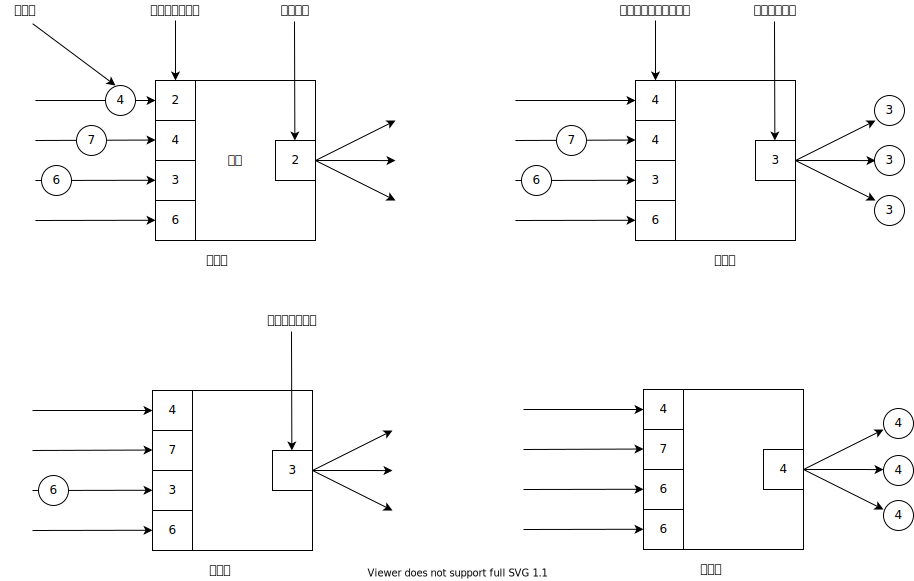
\includegraphics[width=.8\textwidth]{32.pdf}
  \caption{多流转换水位线传播机制}
\end{figure}

\begin{itemize}
  \item 分流:水位线复制然后广播到下游的所有并行子任务中去。
  \item 合流:选择水位线数组中的最小的水位线来更新逻辑时钟。
\end{itemize}

\section{水位线设置的最佳实践}

\begin{itemize}
  \item 在尽量靠近数据源的地方设置水位线(assignTimestampsAndWatermarks)
  \item assignTimestampsAndWatermarks前面的算子的并行度最好是1
\end{itemize}

\section{Kafka水位线设置}

数据源的并行度等于Kafka主题的分区数量。

插入水位线之前的所有算子的并行度和Kafka主题的分区数量一致。

\section{如何处理迟到数据}

到达的数据的时间戳小于当前算子的水位线,就是迟到数据。只有在使用事件时间的情况下,才会存在迟到元素。对于处理时间来说,不存在迟到数据。

处理迟到数据的策略:

\begin{enumerate}
  \item 默认策略:直接丢弃掉迟到数据。当数据到达以后,发现所属窗口已经闭合计算并销毁了,那么数据就被直接丢弃了。
    \begin{itemize}
      \item 如果来的数据是迟到数据,但是所属窗口还在,那么数据可以进入窗口。
      \item 如果来的数据是迟到数据,但所属窗口已经销毁,那么数据被丢弃。
    \end{itemize}
  \item 将迟到数据发送到侧输出流中去。侧输出流是不同于主流输出的旁路输出流,可以向侧输出流发送任意数据。
  \item 使用迟到元素更新窗口计算结果。也就是当水位线到达窗口结束时间的时候,触发窗口计算,但不销毁窗口,而是选择再等待迟到元素一段时间。
    \begin{itemize}
      \item .allowedLateness(Time.seconds(5)):窗口会等待5秒钟的迟到事件
      \item 窗口真正销毁:水位线 $\ge$ 窗口结束时间 + allowedLateness
      \item 窗口的第一次触发计算:水位线 $\ge$ 窗口结束时间,触发计算完以后窗口不会被销毁
    \end{itemize}
\end{enumerate}

\textbf{处理迟到数据的作用}:将迟到数据保存下来,然后统计一下每天有多少迟到数据,然后方便我们调整最大延迟时间的设置,改进计算结果的正确性。

\chapter{多流合并}

Flink的多流合并的机制是以FIFO的方式合并多条流。

\begin{itemize}
  \item union
    \begin{itemize}
      \item 多条流的元素类型必须一样
      \item 可以合并多条流
    \end{itemize}
  \item connect
    \begin{itemize}
      \item 只能合并两条流
      \item 两条流的元素的类型可以不一样
      \item DataStream API
      \begin{itemize}
        \item CoMapFunction<IN1, IN2, OUT>
        \begin{itemize}
          \item map1
          \item map2
        \end{itemize}
        \item CoFlatMapFunction<IN1, IN2, OUT>
        \begin{itemize}
          \item flatMap1
          \item flatMap2
        \end{itemize}
      \end{itemize}
      \item 底层API
      \begin{itemize}
        \item CoProcessFunction<IN1, IN2, OUT>
        \begin{itemize}
          \item processElement1
          \item processElement2
          \item onTimer
          \item 状态变量
        \end{itemize}
      \end{itemize}
      \item 应用场景
        \begin{itemize}
          \item 一条流进行keyBy,另一条流broadcast,使的所有的逻辑分区都能和同一条流进行JOIN。
          \item 两条流都进行keyBy,将来自两条流的相同key的数据合并在一起处理,也就是说,将来自两条流的相同key的数据放在一个逻辑分区中做处理。
          \begin{minted}[frame=single]{sql}
            SELECT * FROM A JOIN B ON A.key=B.key;
          \end{minted}
        \end{itemize}
    \end{itemize}
\end{itemize}

\chapter{Flink中的状态变量}

\begin{itemize}
  \item 算子状态(Operator State)
  \begin{itemize}
    \item 算子状态的作用范围限定为算子的并行子任务,由同一并行子任务所处理的所有数据都可以访问到相同的状态。
    \item 算子状态对于同一并行子任务而言是共享的。
    \item 算子状态不能由相同或不同算子的另一个并行子任务访问。
  \end{itemize}
  \item 键控状态(Keyed State)
  \begin{itemize}
    \item 键控状态是根据输入数据流中定义的key来维护和访问的。
    \item Flink为每个key维护一个状态实例,并将具有相同key的所有数据,都分区到算子的同一个并行子任务中,这个任务会维护和处理这个key对应的状态。
    \item 当任务处理一条数据时,它会自动将状态的访问范围限定为当前数据的key。
    \item 键控状态的底层维护方式是在并行子任务中维护一张HashMap。
  \end{itemize}
  \item 窗口状态(Windowed State):作用域是每个窗口。
  
  案例:使用迟到数据更新窗口计算结果。
\end{itemize}

\begin{figure}[htbp]
  \centering
  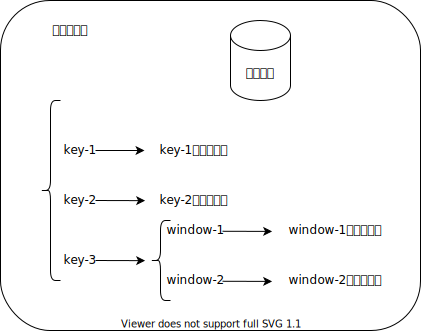
\includegraphics[width=.8\textwidth]{33.pdf}
  \caption{各种状态变量的作用域示意图}
\end{figure}

\section{Flink中的状态管理}

\subsection{状态后端}

\begin{itemize}
  \item 每传入一条数据,有状态的算子任务都会读取和更新状态
  \item 由于有效的状态访问对于处理数据的低延迟至关重要,因此每个并行任务都会在本地维护其状态,以确保快速的状态访问
  \item 状态的存储、访问以及维护,由一个可插入的组件决定,这个组件就叫做状态后端(state backend)
  \item 状态后端主要负责两件事:本地的状态管理,以及将检查点(checkpoint)状态写入远程存储(HDFS、RocksDB、文件系统之类的)
\end{itemize}

\subsection{选择一个状态后端}

\begin{itemize}
  \item MemoryStateBackend(默认)
    \begin{itemize}
      \item 内存级的状态后端,会将键控状态作为内存中的对象进行管理,将它们存储在TaskManager的JVM堆上,而将checkpoint存储在JobManager的内存中
      \item 特点:快速、低延迟,但不稳定
    \end{itemize}
  \item FsStateBackend
    \begin{itemize}
      \item 将checkpoint存到远程的持久化文件系统(FileSystem)上,而对于本地状态,跟MemoryStateBackend一样,也会存在TaskManager的JVM堆上
      \item 同时拥有内存级的本地访问速度,和更好的容错保证
    \end{itemize}
  \item RocksDBStateBackend
    \begin{itemize}
      \item 将所有状态序列化后,存入本地的RocksDB中存储。
      \item RocksDB是一个硬盘KV数据库。
    \end{itemize}
\end{itemize}

\chapter{Flink的容错机制}

\section{Flink程序如何从检查点恢复程序}

\begin{figure}[htbp]
  \centering
  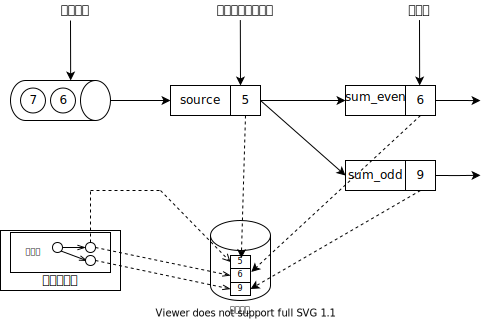
\includegraphics[width=.8\textwidth]{35.pdf}
  \caption{快照}
\end{figure}

\begin{itemize}
  \item Flink故障恢复机制的核心,就是应用状态的一致性检查点。
  \item 有状态流应用的一致检查点,其实就是所有并行子任务的状态,在某个时间点的一份拷贝(一份快照)。
  \item 上游是一个可重置读取位置的持久化设备(例如Kafka)。
\end{itemize}

\begin{figure}[htbp]
  \centering
  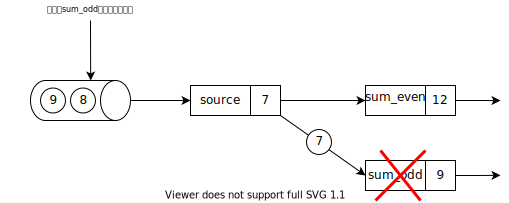
\includegraphics[width=.8\textwidth]{36.pdf}
  \caption{故障}
\end{figure}

\clearpage
\begin{figure}[htbp]
  \centering
  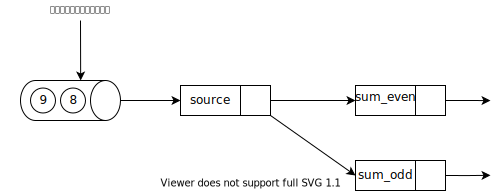
\includegraphics[width=.8\textwidth]{37.pdf}
  \caption{第一步:重启}
\end{figure}

\begin{figure}[htbp]
  \centering
  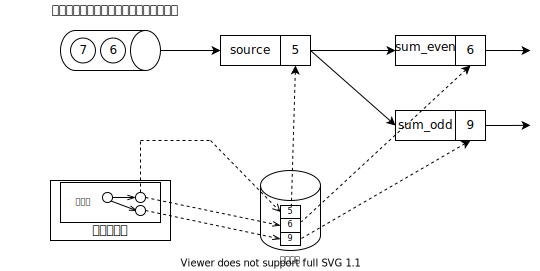
\includegraphics[width=.8\textwidth]{38.pdf}
  \caption{第二步:从检查点文件恢复状态}
\end{figure}

\begin{figure}[htbp]
  \centering
  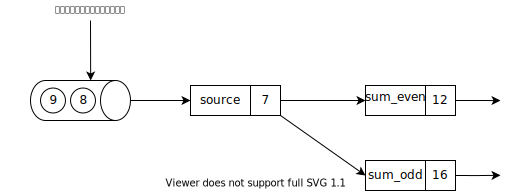
\includegraphics[width=.8\textwidth]{39.pdf}
  \caption{第三步:继续处理数据}
\end{figure}

\section{Flink如何保存检查点}

\textbf{保存检查点的算法}

\begin{itemize}
  \item 同步的思想:暂停应用,保存状态到检查点,再重新恢复应用(Spark Streaming)
  \item 异步的思想(Flink的改进实现)
  \begin{itemize}
    \item 基于Chandy-Lamport算法的异步分布式快照算法
    \item 将检查点的保存和数据处理分离开,不暂停整个应用
  \end{itemize}
\end{itemize}

\chapter{端到端一致性}

\section{状态一致性分类}

\begin{itemize}
  \item AT-MOST-ONCE(最多一次)
  \begin{itemize}
      \item 当任务故障时,最简单的做法是什么都不干,既不恢复丢失的状态,也不重播丢失的数据。at-most-once语义的含义是最多处理一次事件。例如:UDP,不提供任何一致性保障
  \end{itemize}
  \item AT-LEAST-ONCE(至少一次)
  \begin{itemize}
      \item 在大多数的真实应用场景,我们希望不丢失事件。这种类型的保障称为at-least-once,意思是所有的事件都得到了处理,而一些事件还可能被处理多次。
  \end{itemize}
  \item EXACTLY-ONCE(精确一次)
  \begin{itemize}
      \item 恰好处理一次是最严格的保证,也是最难实现的。恰好处理一次语义不仅仅意味着没有事件丢失,还意味着针对每一个数据,内部状态仅仅更新一次。
  \end{itemize}
\end{itemize}

\section{端到端状态一致性}

\begin{itemize}
  \item 目前我们看到的一致性保证都是由流处理器实现的,也就是说都是在Flink流处理器内部保证的;而在真实应用中,流处理应用除了流处理器以外还包含了数据源(例如Kafka)和输出到持久化系统
  \item 端到端的一致性保证,意味着结果的正确性贯穿了整个流处理应用的始终;每一个组件都保证了它自己的一致性
  \item 整个端到端的一致性级别取决于所有组件中一致性最弱的组件
\end{itemize}

\section{端到端EXACTLY-ONCE一致性保障}

\begin{itemize}
  \item 内部保证—checkpoint(分布式异步快照算法)
  \item Source端—可重设数据的读取位置(Kafka,FileSystem)
  \item Sink端—从故障恢复时,数据不会重复写入外部系统
  \begin{itemize}
      \item 幂等写入
      \item 事务写入
  \end{itemize}
\end{itemize}

\section{幂等写入}

所谓幂等操作,是说一个操作,可以重复执行很多次,但只导致一次结果更改,也就是说,后面再重复执行就不起作用了。

\section{事务写入}

\begin{itemize}
  \item 事务(Transaction)
  \begin{itemize}
      \item 应用程序中一系列严密的操作,所有操作必须成功完成,否则在每个操作中所作的所有更改都会被撤消(ACID)
      \item 具有原子性:一个事务中的一系列的操作要么全部成功,要么一个都不做
  \end{itemize}
  \item 实现思想:构建的事务对应着checkpoint,等到checkpoint真正完成的时候,才把所有对应的结果写入Sink系统中
  \item 实现方式
  \begin{itemize}
      \item 预写日志(WAL,Write Ahead Log)(只能保证at-least-once)
      \item 两阶段提交(Two Phase Commit,2PC)(可以保证exactly-once)
  \end{itemize}
\end{itemize}

\section{预写式日志}

\begin{itemize}
  \item 把结果数据(也就是要输出的数据)先缓存到状态后端,然后在收到检查点完成的通知时,一次性写入Sink系统(状态后端 $\rightarrow$ 下游设备)(万一写到中间的时候挂掉了呢?WAL只能保障at-least-once)
  \item 简单易于实现,由于数据提前在状态后端中做了存储,所以无论什么样的下游设备,都能用这种方式一批搞定
  \item DataStream API提供了一个模板类:GenericWriteAheadSink,来实现这种预写式日志的Sink。
\end{itemize}

\section{两阶段提交}

\begin{itemize}
  \item 对于每个检查点,Sink任务会启动一个事务(下游设备的事务,比如MySQL,Kakfa),并将接下来所有接收的数据添加到事务里
  \item 然后将这些数据写入外部Sink系统,但不提交它们——这时只是“预提交”
  \item 当它收到检查点完成的通知时,它才正式提交事务,实现结果的真正写入
  \begin{itemize}
      \item 这种方式真正实现了Exactly-Once,它需要一个提供事务支持的外部Sink系统。Flink提供了TwoPhaseCommitSinkFunction接口。
      \item 有可能在一段时间内看不到Sink的结果
  \end{itemize}
\end{itemize}

\section{总结}

\begin{center}
  \begin{tabular}{|l|l|l|}
  \hline
  \diagbox[width=4cm]{sink}{source} & 不可重置的源 & 可重置的源 \\
  \hline
  any sink & at-most-once & at-least-once \\
  \hline
  幂等性sink & at-most-once & exactly-once \\
  \hline
  预写式日志sink & at-most-once & at-least-once \\
  \hline
  2PC sink & at-most-once & exactly-once \\
  \hline
  \end{tabular}%
\end{center}

\section{Kafka $\rightarrow$ Flink $\rightarrow$ Kafka端到端一致性}

\begin{itemize}
  \item 内部—利用检查点机制,把状态存盘(HDFS),发生故障的时候可以恢复,保证内部的状态一致性。
  \item source—FlinkKafkaConsumer作为source,可以将偏移量保存下来,如果后续任务出现了故障,恢复的时候可以由连接器重置偏移量,重新消费数据,保证一致性。
  \item sink—FlinkKafkaProducer作为sink。
\end{itemize}

\subsection{两阶段提交步骤}

\begin{enumerate}
  \item 第一条数据来了之后,开启一个Kafka的事务(transaction),正常写入Kafka分区日志但标记为未提交,这就是“预提交”
  \item JobManager触发checkpoint操作,barrier从source开始向下传递,遇到barrier的算子将状态存入状态后端,并通知JobManager
  \item Sink连接器收到barrier,保存当前状态,存入checkpoint,通知JobManager,并开启下一阶段的事务,用于提交下个检查点的数据
  \item JobManager收到所有任务的通知,发出确认信息,表示checkpoint完成
  \item Sink任务收到JobManager的确认信息,正式提交这段时间的数据
  \item 外部Kafka关闭事务,提交的数据可以正常消费了
\end{enumerate}

\chapter{背压问题}

背压问题的本质:单位时间缓冲区入队列的数据量,大于缓冲区出队列的数据量。

\begin{enumerate}
  \item 减慢入队列(生产者)的速度
  \item 加快出队列(消费者)的速度
  \item 增大缓冲区队列的大小
  \item 消费者告诉生产者自己目前能消费多少(信任度)
\end{enumerate}

下游算子会向上有算子发送一个消息,告诉上游算子自己的接收缓冲区能接收多少数据,当上游算子的缓冲区攒够 $\le$ 下游算子的接收缓冲区能接收的数据量,就发送下去。

例如:

下游算子的接收缓冲区的大小是4,但目前只有3个元素,也就是说还能接收1个元素,那么会发送一条消息给上游算子,告诉上游算子自己的缓冲区还有1个空位,这样当上游算子的发送缓冲区里有1条数据,直接发送给下游算子的接收缓冲区。

\textbf{信任度算法}

信任度:下游算子的接收缓冲区还能接收多少条数据。

\textbf{基于信用度的流量控制}

通过网络连接来发送每条数据的效率很低,会导致很大的开销。为了充分利用网络连接的带宽,就需要进行缓冲了。在流处理的上下文中,缓冲的一个缺点是会增加延迟,因为数据需要在缓冲区中进行收集,而不是立即发送。

Flink实现了一个基于信任度的流量控制机制,其工作原理如下。接收任务授予发送任务一些“信任度”(credit),也就是为了接收其数据而保留的网络缓冲区数。当发送者收到一个信任度通知,它就会按照被授予的信任度,发送尽可能多的缓冲数据,并且同时发送目前积压数据的大小——也就是已填满并准备发送的网络缓冲的数量。接收者用保留的缓冲区处理发来的数据,并对发送者传来的积压量进行综合考量,为其所有连接的发送者确定下一个信用度授权的优先级。

基于信用度的流控制可以减少延迟,因为发送者可以在接收者有足够的资源接受数据时立即发送数据。此外,在数据倾斜的情况下,这样分配网络资源是一种很有效的机制,因为信用度是根据发送者积压数据量的规模授予的。因此,基于信用的流量控制是Flink实现高吞吐量和低延迟的重要组成部分。

\chapter{有限状态机}

\chapter{竞争状态和锁机制}

\end{document}